\chapter{Funktionen}\label{ch:K04_Functions}

\section{Eigene Funktionen in Python definieren}

Sie kennen bereits die Funktionen \lstinline|print| sowie \lstinline|t.forward| und haben diese auch schon mehrmals selbst verwendet. In diesem Kapitel werden Sie lernen, wie Sie eigene Funktionen in Python definieren und schliesslich sinnvoll verwenden können. Funktionen helfen enorm dabei, Programme leserlicher, kürzer, effizienter und wartbarer zu machen. Funktionen sind deshalb aus modernen Programmen kaum wegzudenken.

\begin{myexample}\label{myexample:flower}
Wir betrachten nochmals den Code aus \cref{myexercise:Blume}:

\lstinputlisting[language=Python,caption=\texttt{blume.py}]{Grundlagen_Info/00_Programmieren/Skript/Code/K02_Intro/blume.py}

Die Blume entsteht durch das wiederholte Zeichnen eines Quadrats, wobei sich die Turtle nach jedem gezeichneten Quadrat um $36$ Grad rotiert.
Wir könnten den Code leserlicher machen, indem wir zunächst eine Funktion \lstinline|quadrat()| definieren, welche lediglich ein Quadrat zeichnet. Danach definieren wir eine weitere Funktion \lstinline|quadrat_blume|, welche die Funktion \lstinline|quadrat| insgesamt 10 Mal aufrufen wird:

\begin{minipage}{\linewidth}
	\begin{figure}[H] % not really a figure, just acts as non-floating container
		\begin{lstlisting}[escapechar=!, numbers=left]
import turtle as t

def !\colorbox{HotPink}{quadrat()}!: !\tikzmark{to2ex}!
    for _ in range(4):
        t.fd(100)
        t.rt(360/4)

def !\colorbox{CornflowerBlue}{quadrat\_blume()}!:!\tikzmark{to1ex}! 
    for _ in range(10):
        !\colorbox{HotPink}{quadrat()}! !\tikzmark{from2ex}!
        t.rt(360/10)

!\colorbox{CornflowerBlue}{quadrat\_blume()}! !\tikzmark{from1ex}!

t.done()
\end{lstlisting}
		\begin{tikzpicture}[overlay,remember picture]
			\draw[CornflowerBlue,-stealth] (from1ex.north) to[out=0, in=0, looseness=2.5] node[fill=CornflowerBlue,rounded corners,font=\sffamily\small,text=white] {\emoji{cook} Aufruf} (to1ex);
			\draw[HotPink,-stealth] (from2ex.north) to[out=0, in=0, looseness=2.5]
			node[fill=HotPink,rounded corners,font=\sffamily\small,text=white] {\emoji{cook} Aufruf} (to2ex);
		\end{tikzpicture}
	\end{figure}
\end{minipage}
Die Erstellung der Definitionen einer Funktion ist vergleichbar mit dem Verfassen eines Kochrezepts (oder eines Bauplans). Die Funktion beschreibt dabei einen Programmablauf, also ein \enquote{Rezept}. Die alleinige Existenz eines Kochrezepts führt natürlich nicht zu einem fertigen Gericht. Dieses entsteht erst bei der Ausführung des Rezepts. Genauso hat in Python die Definition noch keinen Effekt. Der Effekt (die Wirkung der Funktion) erfolgt erst bei ihrem Aufruf (in dem obigen Beispiel erfolgen solche Funktionsaufrufe in den Zeilen 10 und 13).
\end{myexample}


\begin{myoverview}
	% Um eine eigene Funktion zu \lstinline|def|inieren, beginnen wir mit dem Python-Keyword \lstinline|def| gefolgt von einem selbst gewählten Namen (zum Beispiel \lstinline|quadrat| oder \lstinline|meine_funktion|) und Klammern\footnote{Häufig werden hier noch Parameter aufgelistet, siehe \cref{sec:Parameter}.}.
	Innerhalb des eingerückten Bereichs unter \lstinline|def| wird eine Wirkung definiert. Diese Wirkung wird aber erst ausgelöst, wenn die Funktion aufgerufen (und somit der Code ausgeführt) wird!

	Das Schreiben von Definitionen hat mehrere Vorteile:
	\begin{itemize}
		\item Der Code wird \textbf{modular}: Man kann nun einfachere Funktionen schreiben, wie beispielsweise \lstinline|quadrat()|, und komplexere Funktionen, die Unter-Funktionen aufrufen, wie beispielsweise \lstinline|quadrat_blume()|. Auf diese Weise wird ein komplexer Code in einzelne, einfachere Teile (Module) unterteilt.
		\item Der Code wird \textbf{übersichtlicher}: Jede Teil-Aktivität ist eine Funktion
		\item Falls das komplexere Programm nicht das gewünschte Resultat liefert, können wir es \textit{debuggen}, indem wir die einfacheren Funktionen zuerst aufrufen und sicherstellen, dass diese richtig funktionieren.
	\end{itemize}
\end{myoverview}

\begin{myexample}
Die folgende Gegenüberstellung illustriert, wie Funktionen dabei helfen, Programme übersichtlicher zu machen und Struktur in den Code zu bringen:
\begin{figure}[H] % This makes the whole thing float
	\centering
	\begin{minipage}{.4\textwidth}
		\begin{lstlisting}[escapechar=!]
import turtle as t

for _ in range(10):   !\tikzmark{repOuterStart}!
    for _ in range(4):!\tikzmark{repInnerStart}!
        t.fd(100)
        t.rt(360 / 4) !\tikzmark{repInnerEnd}!
    t.fd(360 / 10)    !\tikzmark{repOuterEnd}!

t.done()
  \end{lstlisting}
	\end{minipage}\hfill
	\begin{minipage}{.4\textwidth}
		\begin{lstlisting}[escapechar=!]
import turtle as t

!\tikzmark{repInnerStartTo}!def quadrat():
    for _ in range(4):
        t.fd(100)
!\tikzmark{repInnerEndTo}!        t.rt(360 / 4)

!\tikzmark{repOuterStartTo}!def quadrat_blume():
    for _ in range(10):
        quadrat()
!\tikzmark{repOuterEndTo}!        t.rt(360/10)

quadrat_blume()

t.done()
  \end{lstlisting}

		\begin{tikzpicture}[overlay, remember picture,
				every edge/.append style = { ->, thick, >=stealth, red!70},
				every node/.style={draw=red!50,fill=red!50!white,text=black,rounded corners}]
			\drawBrace{0em}{repInnerStart}{repInnerEnd}{}{.5}{};
			\drawBrace{-.5em}{repInnerStartTo}{repInnerEndTo}{}{.5}{mirror};
			\draw[->, style={thick, >=stealth, red!70}] (repInnerStartrepInnerEnd-coord-arrow) to (repInnerStartTorepInnerEndTo-coord-arrow);
			\drawBrace{1em}{repOuterStart}{repOuterEnd}{}{.75}{};
			\drawBrace{-.5em}{repOuterStartTo}{repOuterEndTo}{}{.25}{mirror};
			\draw[->, style={thick, >=stealth, red!70}] (repOuterStartrepOuterEnd-coord-arrow) to (repOuterStartTorepOuterEndTo-coord-arrow);
		\end{tikzpicture}
	\end{minipage}
	\caption{Vergleich von Schleifen mit Funktionsdefinitionen}
	\label{fig:code-comparison}
\end{figure}
\end{myexample}
Tipps für das Schreiben von Funktionen:
\begin{itemize}
	\item Der Name einer Funktion sollte selbsterklärend und beschreibend sein. Im Idealfall lässt der Name der Funktion schon viel über ihren Effekt erahnen. Beispielsweise ist der Funktionsname \lstinline|quadrat| viel beschreibender als ein nichtssagender Name wie zum Beispiel \lstinline|f|.
	\item
	      Etwas komplexere Tätigkeiten sollten jeweils als eine Funktion definiert werden und damit einen Namen erhalten. So kann beispielsweise das Zeichnen eines Quadrats in einer Funktion \lstinline|quadrat| definiert werden, während das Zeichnen einer Blume in der Funktion \lstinline|quadrat_blume| definiert wird. Diese Funktion kann dann wiederum die Funktion \lstinline|quadrat| aufrufen.
\end{itemize}

\begin{myexercise}
	Führen Sie den folgenden Code zuerst aus und betrachten Sie das Resultat. Schreiben Sie den Code um, indem Sie zwei Funktionen schreiben:

	\begin{enumerate}
		\item \lstinline|viertelkreis|
		\item \lstinline|abgerundetes_quadrat|
	\end{enumerate}

	\begin{lstlisting}
import turtle as t

for _ in range(4):
    for _ in range(9):
        t.fd(4)
        t.lt(10)
    t.fd(100)

t.done()
\end{lstlisting}

	\begin{myanswer}
		\begin{figure}[H]
			\centering
			\begin{minipage}{.4\textwidth}
				\begin{lstlisting}[escapechar=!]
import turtle as t

for _ in range(4):    !\tikzmark{repOuterStart}!
    for _ in range(9):!\tikzmark{repInnerStart}!
        t.fd(4)
        t.lt(10)      !\tikzmark{repInnerEnd}!
    t.fd(100)         !\tikzmark{repOuterEnd}!
\end{lstlisting}
			\end{minipage}\hfill\begin{minipage}{.4\textwidth}
				\begin{figure}[H] % not really a figure, just acts as non-floating container
					\begin{lstlisting}[escapechar=!]
import turtle as t

!\tikzmark{repInnerStartTo}!def viertelkreis():
    for _ in range(9):
        t.fd(4)
!\tikzmark{repInnerEndTo}!        t.lt(10)

!\tikzmark{repOuterStartTo}!def abgerundetes_quadrat():
    for _ in range(4):
        viertelkreis()
!\tikzmark{repOuterEndTo}!        t.fd(100)

abgerundetes_quadrat()

t.done()
\end{lstlisting}
					\begin{tikzpicture}[overlay, remember picture,
							every edge/.append style = { ->, thick, >=stealth, red!70},
							every node/.style={draw=red!50,fill=red!50!white,text=black,rounded corners}]
						\drawBrace{0em}{repInnerStart}{repInnerEnd}{}{.5}{};
						\drawBrace{-.5em}{repInnerStartTo}{repInnerEndTo}{}{.5}{mirror};
						% arrow pointing from one code to other
						\draw[->, style={thick, >=stealth, red!70}] (repInnerStartrepInnerEnd-coord-arrow) to (repInnerStartTorepInnerEndTo-coord-arrow);
						\drawBrace{1em}{repOuterStart}{repOuterEnd}{}{.75}{};
						\drawBrace{-.5em}{repOuterStartTo}{repOuterEndTo}{}{.25}{mirror};
						% arrow pointing from one code to other
						\draw[->, style={thick, >=stealth, red!70}] (repOuterStartrepOuterEnd-coord-arrow) to (repOuterStartTorepOuterEndTo-coord-arrow);
					\end{tikzpicture}
				\end{figure}
			\end{minipage}
		\end{figure}
	\end{myanswer}
\end{myexercise}

\begin{myexercise}
	Packen Sie Ihre Lösung aus \cref{myexercise:Haus} in eine Funktion mit dem Namen \lstinline|haus|. Testen Sie zunächst, ob die  Funktion wirklich das gewünschte Resultat liefert (ein einzelnes Haus), indem Sie die Funktion aufrufen. Schreiben Sie dann eine zweite Funktion \lstinline|haeuserreihe|, welche eine Häuserreihe aus 5 Häusern zeichnet, indem \lstinline|haus| fünfmal aufgerufen wird.

	Ihr Code sollte folgendes Bild ausgeben:
	\begin{figure}[H]
		\centering
		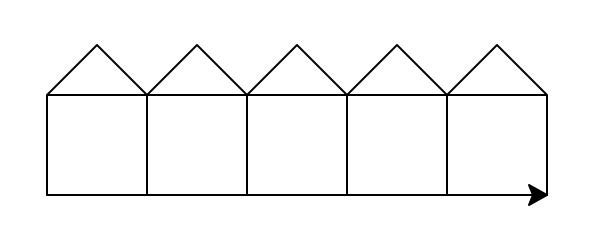
\includegraphics[width=0.3\linewidth]{Grundlagen_Info/00_Programmieren/Skript/Figures/haeuserreihe}
	\end{figure}

	\begin{myanswer}
		Siehe den Code in \cref{ex:local-global}.
	\end{myanswer}
\end{myexercise}

\section{Parameter}\label{sec:Parameter}

Stellen Sie sich vor, Sie wollen drei unterschiedlich grosse Quadrate zeichnen. Sie könnten folgendermassen vorgehen:

\lstinputlisting[language=Python,caption=\texttt{squares\_noparams.py},label=listing:squares_noparams]{Grundlagen_Info/00_Programmieren/Skript/Code/K04_Functions/squares_noparams.py}

Das ging gerade noch! Was jedoch, wenn Sie 20 unterschiedlich grosse Quadrate zeichnen wollen? Brauchen Sie dann 20 Definitionen? Zum Glück nicht, wie Beispiel \cref{ex:params} zeigt.

\begin{myexample}\label{ex:params}
Folgendes Beispiel verwendet einen \textit{Parameter} \texttt{laenge}, um die Länge des Quadrats jedes Mal anzupassen:
\begin{figure}[H] % not really a figure, just acts as non-floating container
	\begin{lstlisting}[escapechar=!, numbers=left]
import turtle as t

def quadrat(!\colorbox{HotPink}{la\tikzmark{arrowTo1}enge}!):
	for _ in range(4):
		t.fd(!\colorbox{HotPink}{la\tikzmark{arrowTo2}enge}!) 
		t.rt(90)

quadrat(!\colorbox{HotPink}{5\tikzmark{arrow1From}0}!)
quadrat(!\colorbox{HotPink}{1\tikzmark{arrow2From}00}!)
quadrat(!\colorbox{HotPink}{1\tikzmark{arrow3From}50}!)
\end{lstlisting}
	\begin{tikzpicture}[overlay,remember picture]
		\draw[CornflowerBlue,-stealth] (arrowTo1.south) to[bend right] (arrowTo2);

		\draw[CornflowerBlue,-stealth] (arrow1From.south) to[out=0, in=10, looseness=2.5] node[right, yshift=-.8cm, fill=CornflowerBlue,text=white,rounded corners] {\emoji{handshake} Übergaben} (arrowTo1);
		\draw[CornflowerBlue,-stealth] (arrow2From.south) to[out=-5, in=20, looseness=2.5] (arrowTo1);
		\draw[CornflowerBlue,-stealth] (arrow3From.south) to[out=0, in=30, looseness=2.5] (arrowTo1);
	\end{tikzpicture}
\end{figure}
\end{myexample}

Funktionen können mehrere (oder auch gar keine) Parameter haben. Ersteres ist besonders nützlich, wenn Sie eine Funktion schreiben wollen, die mehrere Werte benötigt, um ihre Aufgabe zu erfüllen. Zum Beispiel könnte eine Funktion, die ein Vieleck zeichnet, sowohl die Anzahl der Ecken als auch die Farbe des Vielecks benötigen.

\begin{myexample}\label{ex:multiple-params}
In folgendem Beispiel kann nicht nur die Anzahl Ecken, sondern auch die Farbe eines Vielecks übergeben werden.
\lstinputlisting[language=Python,caption=\texttt{farb\_vieleck.py},label=listing:farb_vieleck]{Grundlagen_Info/00_Programmieren/Skript/Code/K04_Functions/farb_vieleck.py}
\begin{figure}[H]
	\centering
	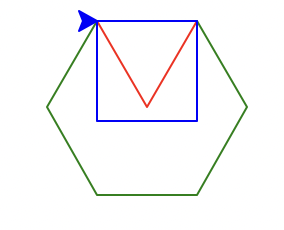
\includegraphics[width=0.2\linewidth]{Grundlagen_Info/00_Programmieren/Figures/mehrere-parameter}
\end{figure}
\end{myexample}

\begin{myoverview}[Begrifflichkeiten bei Python-Funktionen]\label{myoverview:NomenklaturFunktion}
	Wir haben in diesem Kapitel mehrere wichtige Begriffe im Zusammenhang mit Funktionen in Python kennengelernt. Diese Begriffe wollen wir hier anhand eines Beispiels übersichtlich darstellen:
	\begin{lstlisting}
    def produkt(x, y):
        print(x * y)


    produkt(5, 3)
    \end{lstlisting}
	\bigskip
	\begin{description}
		\item[Name der Funktion:] \lstinline|produkt|\\
		      Das ist der Name (Bezeichner) der Funktion, mit dem sie definiert und aufgerufen wird.
		\item[Parameter der Funktion:] \lstinline|x|, \lstinline|y|\\
		      Das sind die Platzhalter in der Funktionsdefinition, die beim Aufruf der Funktion mit Werten (Argumenten) belegt werden.
		\item[Argumente der Funktion:] \lstinline|5|, \lstinline|3|\\
		      Das sind die tatsächlichen Werte, die beim Aufruf an die Funktion übergeben werden.
		\item[Funktionsaufruf:] \lstinline|produkt(5, 3)|\\
		      Das ist der Ausdruck, mit dem die Funktion ausgeführt wird.
		\item[Funktionssignatur:] \lstinline|produkt(x, y)|\\
		      Das ist die Kombination aus dem Funktionsnamen und der Parameterliste, also wie die Funktion definiert ist und wie sie verwendet werden soll.
		\item[Körper der Funktion:] \lstinline|print(x * y)|\\
		      Der Anweisungsblock innerhalb der Funktion. Er definiert, was die Funktion macht.
		\item[Funktion:] \lstinline|def produkt(x, y): ...|\\
		      Das ist die gesamte Struktur, die eine Funktion definiert, einschliesslich des Namens, der Parameter und des Körpers. Typischerweise beginnt sie mit dem Keyword \lstinline|def|, gefolgt von der Funktionssignatur und einem Doppelpunkt, und der Körper ist eingerückt darunter.
	\end{description}

	\medskip
	Die allgemeine Form einer Funktion in Python sieht also so aus:
	\begin{lstlisting}
	# Funktion (Funktionsdefinition)
	def funktionsname(parameter_1, parameter_2, ...):
		# Körper der Funktion
		...
	

	# Funktionsaufruf (nicht mehr Teil der Funktionsdefinition)
	funktionsname(argument_1, argument_2, ...)
	\end{lstlisting}
\end{myoverview}

\begin{myexercise}
	Ändern Sie den Code aus \cref{ex:multiple-params} so ab, dass zusätzlich zur Farbe und der Anzahl Ecken auch noch die \textbf{Stiftdicke} für jedes Vieleck verändert werden kann. Verwenden Sie dazu einen weiteren Parameter sowie die Funktion \lstinline|t.width()|.
\end{myexercise}

\begin{myexercise}
	Erstellen Sie die Funktionen mit den folgenden Signaturen:
	\begin{itemize}
		\item \lstinline|def summiere(x1, x2)|: Berechnet die Summe der zwei Parameter \lstinline|x1| und \lstinline|x2| und gibt das Resultat mittels \lstinline|print| im Terminal aus.
		\item \lstinline|def summe_quadrate(x, y)|: Berechnet die Summe \(x^2 + y^2\) und gibt diese mittels \lstinline{print} im Terminal aus.
	\end{itemize}
\end{myexercise}

\subsection{Lebensdauer (\textit{scope}) einer Variablen}
Im Code aus \cref{ex:params} wird bei \textit{jedem Aufruf} der Definition \lstinline|quadrat| eine neue Variable \texttt{laenge} erstellt, welche nur \textit{innerhalb} der Funktion existiert und welche jedes Mal einen anderen Wert hat. Den Wert erhält die Variable zum Zeitpunkt des \textit{Aufrufs} der Funktion, also auf den Zeilen 8, 9 und 10!

Die Variable \lstinline|laenge| existiert also nur innerhalb der Definition \lstinline|quadrat|. Wenn wir nach Zeile 6 im Hauptprogramm (nicht eingerückt) den Befehl \lstinline|print(laenge)| eingeben würden, würden wir eine Fehlermeldung erhalten, da es die Variable nicht mehr gibt. Parameter sind also immer \textbf{\textit{lokale} Variablen}, ebenso wie Variablen, welche wir innerhalb von Funktionen erstellen. Diese Variablen \enquote{sterben} nach Ausführung der Definition, daher spricht man auch von der Lebensdauer einer Variable, bzw. von deren Reichweite (Englisch: \textit{scope}).

Variablen, welche im Hauptprogramm (nicht eingerückt) erstellt werden, sind sogenannte \textbf{\textit{globale} Variablen}.

\begin{myexercise}\label{ex:local-global}
	Beschreiben Sie, welche der Variablen im unten stehenden Code lokal oder global sind, und welche Variablen auch Parameter sind. Sie sollten insgesamt 5 Variablen finden!
	\lstinputlisting[language=Python,caption=\texttt{houses.py},label=listing:houses]{Grundlagen_Info/00_Programmieren/Skript/Code/K04_Functions/houses.py}

	\begin{myanswer}
		\begin{enumerate}
			\item \lstinline|laenge|: lokale Variable, Parameter der Funktion \lstinline|haus|
			\item \lstinline|anzahl_mauern|: lokale Variable
			\item \lstinline|laenge_pro_haus|: lokale Variable, Parameter der Funktion \lstinline|haeuserreihe|
			\item \lstinline|anzahl_haeuser|: lokale Variable
			\item \lstinline|seitenlaenge|: globale Variable
		\end{enumerate}
	\end{myanswer}
\end{myexercise}

\begin{myexercise}
	Was könnte der Vorteil von \textit{lokalen Variablen} sein?
	\begin{myanswer}
		Falls Sie mehrere Funktionen schreiben, können Sie dieselben Variabelnamen und Parameter-Namen innerhalb der Funktionen verwenden, da diese nichts miteinander zu tun haben. Im Code aus \cref{ex:local-global} hätten wir auch in beiden Funktionen \texttt{laenge} schreiben können.
	\end{myanswer}
\end{myexercise}


\section{Werte zurückgeben mit \texorpdfstring{\lstinline|return|}{return}}
\subsection{Einzelne Funktionen}
Wie Sie bereits wissen, können Definitionen mit Kochrezepten verglichen werden: Sie beschreiben einen Ablauf, ohne diesen auszuführen. Damit der Code einer Funktion ausgeführt wird, müssen Sie die Definition \textbf{aufrufen}: In \cref{ex:multiple-params} wurde dies beispielsweise mit \lstinline|farb_vieleck(3, "red")| gemacht. Erst aufgrund dieser Zeile wurde etwas gezeichnet!

Dies kann nützlich sein, wenn sie eine Aufgabe mehrmals und in unterschiedlichen Varianten ausführen wollen, wie beispielsweise in \cref{ex:multiple-params}.

Eine wichtige Limitation von Definitionen war bisher, dass Sie zwar Dinge berechnen und im Terminal ausgeben konnten, allerdings verschwinden alle Parameter und lokalen Variablen nach der Ausführung einer Funktion.  Dies bedeutet, dass alle Variablen, die wir je in einer Definition erstellt haben, nur in dieser Definition \enquote{lebten}. Wir konnten jedoch nicht mehr auf Parameter oder lokale Variablen zugreifen, nachdem die Funktion beendet wurde.

\begin{myexample}\label{ex:sum-noreturn}
Betrachten Sie folgenden Code. Weshalb führt er zu einer Fehlermeldung?
\begin{lstlisting}[numbers=left]
def summiere(x_1, x_2):
    summe = x_1 + x_2
    
summiere(3, 5)
print(summe)
\end{lstlisting}
Das Terminal gibt folgende Meldung aus: \texttt{[Zeile: 5] NameError: name 'summe' is not defined}. Dies bedeutet, dass der Ausdruck / der Name \lstinline|summe| auf Zeile 5 nicht existiert. Die Fehlermeldung erklärt sich dadurch, dass alle Variablen, die innerhalb einer Definition erstellt werden, nur innerhalb dieser Definition \enquote{\textit{leben}}, also existieren. Dass Variablen mittels dem Befehl \lstinline|return| auch an das Hauptprogramm \enquote{zurückgegeben} werden können, lernen wir in diesem Kapitel.
\end{myexample}

Funktionen können jedoch auch Werte an das Hauptprogramm zurückgeben: In diesem Kapitel lernen wir, wie Funktionen, ähnlich wie \enquote{Sous-Chefs} (Hilfs-Köche) in einer komplexen Küche Zutaten (Parameter) entgegennehmen und Resultate an andere \enquote{Sous-Chefs} (Funktionen) via das Hauptprogramm weitergeben werden können.

Eine Funktion kann man sich vorstellen wie ein Kochrezept, das einige Zutaten entgegennimmt und ein Resultat (Gericht) zurückgibt. Die Zutaten, oder \enquote{Inputs}, werden dabei häufig als \enquote{\textbf{Parameter}} bezeichnet, währenddem das fertige Gericht, oder \enquote{Resultat} häufig als \enquote{\textbf{\lstinline|return|-Wert}} bezeichnet wird. Diese Idee ist in \cref{fig:funktion-einzeln} veranschaulicht.

\begin{figure}[H]
	\centering
	\begin{tikzpicture}
		\drawCube{1}{0}{2}{3}
		\node[fill=blue!50, rounded corners] (input1) at (llD11val){3};
		\node[fill=blue!50, rounded corners] (input2) at (llD21val){12};
		\draw[thick,->] (input1) -- (in11);
		\draw[thick,->] (input2) -- (in12);
		\node[fill=green!50, rounded corners](outVal1) at (5,-.6,3){36};
		\draw[thick,->] (out1) -- (outVal1);
	\end{tikzpicture}
	\caption{Illustration einer Funktion mit Inputs (Parametern) und Outputs (\lstinline|return|-Wert)}
	\label{fig:funktion-einzeln}
\end{figure}

\begin{myexample}
Betrachten Sie nochmals den folgenden, leicht modifizierten Code aus \cref{ex:sum-noreturn}. Wenn wir den Wert mit \lstinline|return| an das Hauptprogramm zurückgeben und in einer Variable (im Hauptprogramm, auf Zeile 5) abspeichern, funktioniert der Code nun: Wir können auch ausserhalb der Funktion \lstinline|summiere()| auf einen Wert zugreifen, welcher innerhalb der Definition berechnet wurde, und diesen potentiell weiterverwenden.
\begin{figure}[H] % not really a figure, just acts as non-floating container
	\begin{minipage}{\linewidth}
		\begin{lstlisting}[numbers=left]
def summiere(x_1, x_2):
    summe = x_1 + x_2
    return (*@\colorbox{RoyalBlue!50}{sum\tikzmark{arrowFromEx01}me}@*)



(*@\colorbox{ForestGreen!50}{re\tikzmark{arrowToEx02}s}@*)=(*@\colorbox{RoyalBlue!50}{summie\tikzmark{arrowToEx01}re(3, 5)}@*)
print(res)
\end{lstlisting}
		\begin{tikzpicture}[overlay,remember picture]
			% Wert zurückgeben
			\draw[RoyalBlue,-stealth, thick] (arrowFromEx01.south) to[bend left] node[align=left, pos=.15, right, fill=RoyalBlue,fill opacity=.5, text opacity=1, text=black,rounded corners] {Wert an das Hauptprogramm zurückgeben...} (arrowToEx01.north);

			\draw[ForestGreen,-stealth, thick] (arrowToEx01.north) to[bend right] node[align=left, pos=.7, above right, fill=ForestGreen,fill opacity=.5, text opacity=1, text=black,rounded corners] {... und Wert in Variable speichern, z.B. \lstinline|res|} (arrowToEx02.north);
		\end{tikzpicture}
	\end{minipage}
\end{figure}

\begin{myattention}
	Man muss sich diesen Code wie folgt vorstellen: Auf Zeile 7 wird die Funktion \lstinline|summiere| aufgerufen, die Werte 3 und 5 werden für die Parameter \lstinline|x1| und \lstinline|x2| übergeben. Zeile 2 berechnet nun die Summe dieser beiden Werte. Auf Zeile 3 wird \textcolor{red}{nicht} die Variable \lstinline|summe| an das Hauptprogramm zurückgegeben, sondern deren Wert (in diesem Fall: 8). Dies ist sehr wichtig: Nur weil wir \lstinline|return summe| schreiben, heisst das nicht, dass wir ausserhalb der Funktion \lstinline|summiere| auf eine Variable \lstinline|summe| zugreifen können. Vielmehr kann man sich vorstellen, dass der blau markierte Bereich auf Zeile 7 nun \enquote{ersetzt} wird durch den Wert 8, welcher vom Unterprogramm an das Hauptprogramm zurückgegeben wird. Zeile 7 liest sich also nach der Ausführung des Unterprogramms so als ob man \lstinline|res = 8| geschrieben hätte. Man könnte selbstverständlich auch einen anderen Variablenname statt \lstinline|res| auswählen, z.B. \lstinline|x|, \lstinline|y|, \lstinline|resultat| (kurz  \lstinline|res|) oder einfach \lstinline|summe|. In letzterem Falle wäre \lstinline|summe| auf Zeile 7 eine globale Variable und somit gänzlich unterschiedlich von der lokalen Variable \lstinline|summe| auf Zeile 2.
\end{myattention}
\end{myexample}

\begin{myexercise}\label{ex:dreieck-return}
	Gegeben seien die Höhe \texttt{h} und die Grundseite \texttt{b} eines Dreiecks. Schreiben Sie eine Funktion \lstinline|flaeche_dreieck(h, b)|, welche den Flächeninhalt dieses Dreiecks berechnet und mit \lstinline|return| zurückgibt. Testen Sie die Funktion mit den Werten \lstinline|h=5| und \lstinline|b=10|, speichern Sie das Resultat in einer Variable \lstinline|result| und geben Sie deren Wert per \lstinline|print| \textit{nach dem Funktionsaufruf} (im Hauptprogramm) aus.

	% Überprüfen Sie die Korrektheit Ihrer Funktion, indem Sie sie auf Moodle hochladen.
	\begin{myanswer}
		\begin{lstlisting}
			def flaeche_dreieck(h, b):
				return h * b / 2

			result = flaeche_dreieck(5, 10)
			print(result)
	\end{lstlisting}
	\end{myanswer}
\end{myexercise}

\begin{myexercise}\label{Wurzelspirale}
	Schreiben Sie ein Programm, dass die Funktion \lstinline|flaeche_dreieck(h, b)| aus \cref{ex:dreieck-return} verwendet, um den Flächeninhalt der folgenden Wurzelspirale zu berechnen.
	\begin{figure}[H]
		\centering
		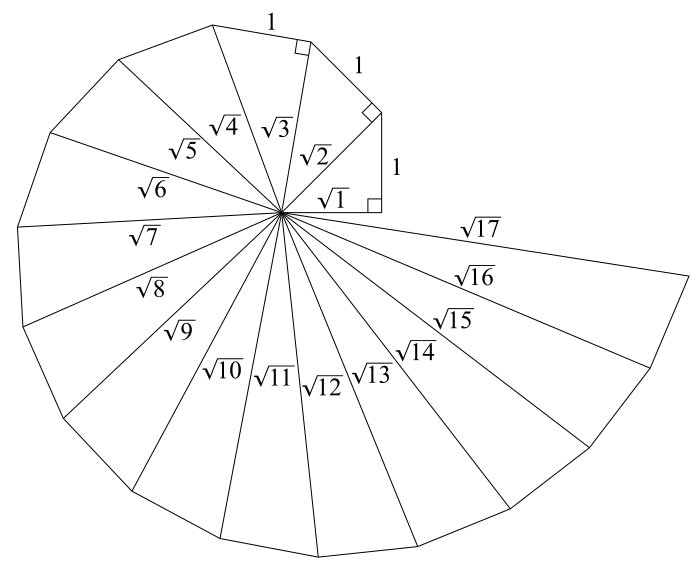
\includegraphics[width=0.3\linewidth]{Grundlagen_Info/00_Programmieren/Skript/Figures/Spiral_of_Theodorus.png}
	\end{figure}
	\begin{myanswer}
		\lstinputlisting[language=Python,caption=\texttt{wurzelspirale.py},label=listing:arithmetic_vars]{Grundlagen_Info/00_Programmieren/Skript/Code/K04_Functions/wurzelspirale.py}
	\end{myanswer}

\end{myexercise}


\begin{myexercise}\label{ex:quadrat-return}
	Gegeben sei eine ganze Zahl \(n\). Schreiben Sie eine Funktion \lstinline|square(n)|, welche das Quadrat von \(n\) berechnet und mit \lstinline|return| zurückgibt. Testen Sie die Funktion mit dem Wert 5, speichern Sie das Resultat in einer Variable \lstinline|result| und geben Sie deren Wert per \lstinline|print| \textit{nach dem Funktionsaufruf} (im Hauptprogramm) aus.

	% Überprüfen Sie die Korrektheit Ihrer Funktion, indem Sie sie auf Moodle hochladen.
	\begin{myanswer}
		\begin{lstlisting}
			def square(n):
				return n * n

			result = square(5)
			print(result)
		\end{lstlisting}
	\end{myanswer}
\end{myexercise}

\begin{myexercise}\label{ex:print-vs-return}
	In welchen Fällen ist es sinnvoller, einen Wert einfach per \lstinline|print| auf der Konsole auszugeben, und wann ist ein \lstinline|return|-Befehl sinnvoller? Ist das Zurückgeben des Werts in \cref{ex:quadrat-return} und \cref{ex:dreieck-return} sinnvoll, oder würde hier auch ein \lstinline|print| reichen?

	\begin{center}
		\begin{tabular}{l|c|c}
			\textbf{Aufgabe}         & \lstinline|print| & \lstinline|return| \\
			\midrule\midrule
			\cref{ex:dreieck-return} &                   &                    \\
			\midrule
			\cref{ex:quadrat-return} &                   &                    \\
		\end{tabular}
	\end{center}

	Begründen Sie Ihre Antwort:
	\begin{myanswer}
		\begin{center}
			\begin{tabular}{l|c|c}
				\textbf{Aufgabe}         & \lstinline|print| & \lstinline|return| \\
				\midrule\midrule
				\cref{ex:dreieck-return} & \faCheckSquare    &                    \\
				\midrule
				\cref{ex:quadrat-return} & \faCheckSquare    &                    \\
			\end{tabular}
		\end{center}
		\lstinline|return|-Ausdrücke ergeben vor allem dann Sinn, wenn mit einem Wert, welcher in einer Funktion berechnet wurde, \textit{ausserhalb der Funktion weitergerechnet} werden soll. In allen anderen Fällen reicht ein \lstinline|print| meist aus. Auch bei \cref{ex:quadrat-return} und \cref{ex:dreieck-return} würde ein einfaches \lstinline|print| reichen.
	\end{myanswer}
\end{myexercise}

\subsection{Mehrere Funktionen}
Wie Sie in \cref{ex:print-vs-return} gesehen haben, ist ein \lstinline|return| in vielen Fällen nicht notwendig, ein einfaches \lstinline|print| reicht in vielen Fällen aus. Wozu kann ein \lstinline|return| eigentlich nützlich sein? Wenn Sie Code schreiben, wird dieser oftmals schnell komplizierter. Somit kann es hilfreich sein, die einzelnen Schritte in Unter-Programme aufzuteilen. Dies erleichtert zudem die \textbf{Modularisierung} und \textbf{Wiederverwendbarkeit} von Code: Beispielsweise könnte eine Funktion, die das Maximum einer Liste berechnet, an verschiedenen Orten in einem längeren Programm mehrmals zum Einsatz kommen.

Zum Vergleich: stellen Sie sich vor, Sie arbeiten in einer edlen Michelin-Sterne-Küche an einem raffinierten Gericht, in das viele Arbeitsschritte involviert sind. Häufig müssen in solchen Restaurants bis zu 200 Schritte pro Gericht ausgeführt werden. Daher könnte es sinnvoll sein, einzelne Aufgaben, wie beispielsweise die Herstellung der Saucen, an Ihre Sous-Chefs zu delegieren, und eine Person zu bestimmen, die das ganze Gericht zusammenfügt. Häufig werden Funktionen genau mit solchen komplexen Aufgaben im Hinterkopf geschrieben. Diese Idee ist in \cref{fig:funktionen-mehrere} illustriert.

\begin{figure}[H]
	% Use the \drawCube macro to draw various cubes
	\centering
	\begin{tikzpicture}
		\drawCube{1}{0}{2}{3}
		% feed input values into a1
		\node[fill=blue!50, rounded corners] (input1) at (llD11val){3};
		\node[fill=blue!50, rounded corners] (input2) at (llD21val){12};
		\draw[thick,->] (input1) -- (in11);
		\draw[thick,->] (input2) -- (in12);
		\node[fill=green!50, rounded corners](outVal1) at (5,-.6,3){36};
		\draw[thick,->] (out1) -- (outVal1);
		\drawCube{2}{5.25}{3}{3}
		\drawCube{3}{10.5}{2}{3}
		\draw[thick,->,rounded corners] (out1) -- ++(0,-3.25,0) -- ++(3.15,0,0)node[below]{\lstinline{return out1}} -- ++(4.65,0,0) -- (in31);
	\end{tikzpicture}
	\caption{Illustration einer Code-Struktur, bei welcher mehrere Funktionen zusammenarbeiten}
	\label{fig:funktionen-mehrere}
\end{figure}

In \cref{fig:funktionen-mehrere} haben wir eine Funktion \lstinline|a1|, die zwei Parameter entgegennimmt (\lstinline|x1| und \lstinline|x2|). Mit diesen Parametern macht sie etwas (z.B. die Summe berechnen, ein Quadrat zeichnen oder irgend eine sonstige Aufgabe) und gibt danach einen neuen, berechneten Wert \lstinline|a1| zurück. Dieser kann im Hauptprogramm abgespeichert und an andere Funktionen weitergegeben werden, beispielsweise an die Funktion \lstinline|a3|.

\begin{myexample}
Stellen Sie sich vor, Sie arbeiten für einen Supermarkt und sollten den Preis Ihrer Produkte berechnen. Sie kaufen Ihre Artikel bei einem Grossverteiler ein, daher erhalten Sie auf alle Produkte 10 \% Rabatt. Der Grossverteiler befindet sich im Ausland, Sie müssen also noch 7 \% Mehrwertsteuer hinzufügen. Der Grossverteiler gibt Ihnen den Original-Preis Ihrer Waren \textit{vor} Rabatt und \textit{vor} Mehrwertsteuer.

Folgender Code berechnet den Endpreis, für den Sie ihre Waren verkaufen werden, indem folgende zwei Funktionen aufgerufen werden:
\begin{enumerate}
	\item \lstinline|berechne_rabatt| berechnet den Preis nach Abzug eines Rabatts für ein Produkt.
	\item \lstinline|berechne_gesamtpreis| ruft \lstinline|berechne_rabatt| auf und fügt zum rabattierten Preis die Mehrwertsteuer hinzu.
\end{enumerate}

\begin{minipage}{\linewidth}
	\begin{figure}[H] % not really a figure, just acts as non-floating container
		\begin{lstlisting}
def berechne_rabatt(preis, rabatt_prozent):
    rabatt = preis * (rabatt_prozent / 100)
    (*@\colorbox{CornflowerBlue}{return preis - \tikzmark{arrowFromEx11} rabatt}@*) # Gibt den Preis nach Abzug des Rabatts zurück


def berechne_gesamtpreis(preis, rabatt_prozent, mwst_prozent):
    (*@\colorbox{CornflowerBlue}{rabatt\tikzmark{arrowToEx11}preis}@*) = berechne_rabatt(preis, rabatt_prozent)
    mwst = rabattpreis * (mwst_prozent / 100)
    return (*@\colorbox{CornflowerBlue}{rabattpre\tikzmark{arrowFromEx12}is + mwst}@*)  # Gibt den Gesamtpreis inklusive Mwst. zurück


# Anwendung
preis = 100  # Basispreis in CHF
rabatt_prozent = 10  # Rabatt in %
mwst_prozent = 7.7  # Mehrwertsteuer in %

(*@\colorbox{CornflowerBlue}{endp\tikzmark{arrowToEx12}reis}@*) = berechne_gesamtpreis(preis, rabatt_prozent, mwst_prozent)
print("Der Endpreis nach Rabatt und Mehrwertsteuer ist:", endpreis)
\end{lstlisting}
		\begin{tikzpicture}[overlay,remember picture]
			% Wert zurückgeben
			\draw[red,-stealth] (arrowFromEx11.north) to[bend left] node[pos=.3, right, fill=RoyalBlue,fill opacity=.5, text opacity=1, text=black,rounded corners] {Wert zurückgeben (und speichern)} (arrowToEx11);
			\draw[red,-stealth] (arrowFromEx12.north) to[bend left] node[pos=.2, right, fill=RoyalBlue, fill opacity=.5, text opacity=1, text=black,rounded corners] {Wert zurückgeben  (und speichern)} (arrowToEx12);
		\end{tikzpicture}
	\end{figure}
\end{minipage}
\end{myexample}


Mit folgendem Code können wir die Turtle eine Spirale aus mehreren Vielecken zeichnen lassen:

\begin{minipage}{.65\textwidth}
	\lstinputlisting[language=Python,caption=\texttt{spirale\_kreis.py}]{Grundlagen_Info/00_Programmieren/Skript/Code/K04_Functions/spirale_kreis.py}
\end{minipage}
\begin{minipage}{.25\textwidth}
	\begin{figure}[H]
		\centering
		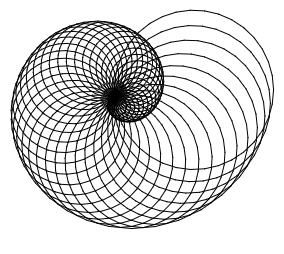
\includegraphics[keepaspectratio, width=\textwidth]{Grundlagen_Info/00_Programmieren/Figures/spirale.png}
	\end{figure}
\end{minipage}

\begin{myexample}
Leider ist unsere Turtle etwas müde und sollte nicht zu viel laufen. Daher möchten wir fortlaufend die Gesamtdistanz berechnen, um am Ende herauszufinden, ob unsere Turtle zu viel Strecke zurückgelegt hat. Dies können wir tun, indem wir die Funktion einen Wert zurückgeben lassen:
\begin{lstlisting}
import turtle as t

def vieleck(umfang, ecken):
    for _ in range(ecken):
        t.fd(umfang/ecken)
        t.rt(360/ecken)

def vieleck_muster(umfang, ecken):
	(*@\colorbox{CornflowerBlue}{gesamtdistanz=0}@*)
    for _ in range(60):
        vieleck(umfang, ecken)
        (*@\colorbox{CornflowerBlue}{gesamtdistanz+=umfang}@*)
        umfang-=10
        t.rt(10)
    (*@\colorbox{CornflowerBlue}{return gesamtdistanz}@*)
    
(*@\colorbox{CornflowerBlue}{gesamtdistanz = }@*)vieleck_muster(600,35)
(*@\colorbox{CornflowerBlue}{print(gesamtdistanz)}@*)
\end{lstlisting}


\end{myexample}


\begin{myexercise}\label{ex:notenskala}
	Schreiben Sie eine Python-Funktion \lstinline|def notenskala(maxPunkte, erreichtePunkte)|, welche die erreichte Note in Abhängigkeit der maximal möglichen Punktzahl und der erreichten Punktzahl berechnet und per \lstinline|return| zurückgibt. Verwenden Sie dafür die folgende Formel:

	\[ \text{\texttt{note}} = \frac{\text{\texttt{erreichtePunkte}}}{\text{\texttt{maxPunkte}} }\cdot 5 + 1 \]
	\begin{myanswer}
		\begin{lstlisting}
def notenskala(maxPunkte, erreichtePunkte):
    return 5 *erreichtePunkte / maxPunkte + 1
\end{lstlisting}
	\end{myanswer}
\end{myexercise}

\begin{myexercise}
	Schreiben Sie ein Programm, das Notenschnitte berechnet. Als erstes soll das Programm den Nutzer Fragen, wie viele Prüfungen stattgefunden haben. Anschliessend soll der Benutzer für jede Prüfung die erreichte und die maximale Punktzahl eingeben.

	Das Programm gibt dann die einzelnen Prüfungsnoten (berechnet mit der Funktion aus \cref{ex:notenskala} und den Gesamtschnitt im Terminal aus.
	\begin{myanswer}
		\lstinputlisting[language=Python,caption=\texttt{notenschnitt.py},label=listing:arithmetic_vars]{Grundlagen_Info/00_Programmieren/Skript/Code/K04_Functions/notenschnitt.py}
	\end{myanswer}

\end{myexercise}


\begin{myexercise}[Formel 1 \emoji{chequered-flag}]\label{ex:f1}
	Ein Formel-1-Auto fährt eine bestimmte Strecke in einer bestimmten Zeit. Schreiben Sie eine Funktion \lstinline|durchschnittsgeschwindigkeit(strecke_km, zeit_min)|, die Strecke in Kilometern und Zeit in Minuten als Eingabe erhält und die durchschnittliche Geschwindigkeit in km/h per \lstinline|return| zurückgibt.

	Formel: Durchschnittsgeschwindigkeit = Strecke (km) / Zeit (h)

	\begin{myanswer}
		\lstinputlisting[language=Python,caption=\texttt{f1\_avg\_speed.py}]{Grundlagen_Info/00_Programmieren/Skript/Code/K04_Functions/f1_avg_speed.py}
	\end{myanswer}
\end{myexercise}

\begin{myexercise}[Boxenstopp \emoji{fuelpump}]
	Ein Formel-1-Rennteam möchte die Gesamtzeit eines Rennens inklusive Boxenstopps berechnen. Gegeben sind die Gesamtstrecke in Kk, die Durchschnittsgeschwindigkeit in km/h, die Anzahl Stopps sowie die Dauer pro Stopp in Sekunden.

	Schreiben Sie zwei Funktionen:

	\lstinline|def fahrzeit_ohne_stopps(strecke, kmh)|: Berechnet die reine Fahrzeit in Sekunden und gibt diese per \lstinline|return| zurück.

	\lstinline|def gesamtzeit(strecke, kmh, stopps, stoppdauer)|: Berechnet zuerst die Fahrzeit ohne Stopps (mit der ersten Funktion) und berechnet dann die Gesamtzeit mit Stopps, indem zur Fahrzeit ohne Stopps die Anzahl Boxenstopps mal die Dauer eines Boxenstopps (in Sekunden) hinzugefügt wird. Das Resultat soll ebenfalls per \lstinline|return| zurückgegeben werden.

	Formel 1: Fahrzeit (Sekunden) = Strecke (km) / Geschindigkeit (km/h) * 3600

	Formel 2: Gesamtzeit (Sekunden) = Fahrzeit + (Anzahl Stopps $\times$ Stoppdauer)

	\textbf{Tipp 1}: Schreiben Sie den Code zuerst in VS Code und testen sie ihn erst nachher auf Moodle.

	\textbf{Tipp 2}: Schreiben Sie zuerst die erste Funktion und testen Sie diese mit folgenden Testwerten: Geschwindigkeit = 210 km/h, Strecke = 305 km. Das Resultat sollte sein: 5228.57 Sekunden. Schreiben Sie erst danach die zweite Definition, und rufen Sie darin die erste Definition auf.

	\begin{myanswer}
		\lstinputlisting[language=Python,caption=\texttt{f1\_pitstops.py}]{Grundlagen_Info/00_Programmieren/Skript/Code/K04_Functions/f1_pitstops.py}
	\end{myanswer}
\end{myexercise}

% \section{Weitere Aufgaben}
% % \subsection{Level 1}
% % \subsection{Level 2}
% % \subsection{Level 3}
% \begin{mychallenge}\label{mychallenge:kaufpreis_haus}
% Sie wollen ein Haus in der Schweiz kaufen. Der Kaufpreis beträgt $k$ Franken. Sie kaufen das Haus mit $E$ Franken Ihres gesparten Geldes (Eigenkapital) und der Restbetrag wird durch die Aufnahme einer Hypothek von $h := k - E$ Franken gedeckt. 

% Die Tragbarkeitsrechnung in der Schweiz prüft, ob die Kosten einer Immobilie langfristig finaziell tragbar (bezahlbar) sind. Banken und andere Kreditinstitute verwenden diese (sehr grobe) Berechnung, um sicherzustellen, dass Sie Ihre Hypothek auch dann noch bezahlen könnten, falls die Zinsen steigen würden. Als Faustregel gilt, dass die jährlichen (kalkulatorischen\footnote{Der Begriff \textit{Kalkulatorisch} bedeutet in diesem Zusammenhang, dass dieser Betrag nach bestimmten Vorgaben berechnet wird und überhaupt nicht den tatsächlichen Kosten entsprechen muss.}) Wohnkosten nicht mehr als $1 / 3$ Ihres \textcolor{ForestGreen}{Bruttojahreseinkommens} ($b$) ausmachen dürfen.

% Die kalkulatorischen jährlichen Wohnkosten setzten sich als die Summe der folgenden drei Positionen zusammen:
% \begin{itemize}
% 	\item \textcolor{NavyBlue}{Kalkulatorischer Zins}: $5$ Prozent des Hypothekenbetrags $h$, also $5$ Prozent von $k - E$
% 	\item \textcolor{Magenta}{Nebenkosten}: $1$ Prozent des Kaufpreises $k$
% 	\item \textcolor{Red}{Amortisation}: Falls die aufgenommene Hypothek grösser als $2/3$ des Kaufpreises $k$ ist, muss der darüberliegende Betrag $h - (2 / 3) k$ nach $15$ Jahren zurückbezahlt sein. Die Bank rechnet also hierführ mit jährlichen Kosten $a$ für die Amortisation von
% 	\begin{align*}
% 		a := \frac{h - (2 / 3) k}{15} = \frac{(k - E) - (2 / 3) k}{15} 
% 	\end{align*}
% 	und mit $a := 0$, falls die Hypothek $2 / 3$ des Kaufpreises nicht übersteigt.
% \end{itemize}
% Zusammengefasst muss also die Ungleichung
% \begin{align*}
% 	\frac{\text{\textcolor{ForestGreen}{Brutto-Jahreseinkommen}}}{3} \geq \text{\textcolor{NavyBlue}{Kalkulatorischer Zins}} + \text{\textcolor{Magenta}{Nebenkosten}} + \text{\textcolor{Red}{Amortisation}}
% \end{align*}
% oder anderst geschrieben
% \begin{align*}
% 	b / 3 \geq 0.05(k - E) + 0.01k + \max\lrc{0, (k/3 - E) / 15}
% \end{align*}
% erfüllt sein. Wir wollen unsere Berechnung möglichst allgemein halten und ersetzen die kalkulatorische Hypothekenrate von $0.05$ durch die positive Variable $\alpha$ und die kalkulatorische Nebenkostenrate $0.01$ durch die positive Variable $\beta$:
% \begin{align}\label{eq:Ungleichung_k}
% 	b / 3 \geq \alpha (k - E) + \beta k + \max\lrc{0, (k/3 - E) / 15}.
% \end{align}

% Nun gibt es für den Kaufpreis $k$ noch eine weitere Zusatzbedingung: \textbf{Der Kaufpreis darf nicht höher sein als das Fünffache des Eigenkapitals}.

% \begin{enumerate}
% 	\item Lösen Sie die Ungleichung nach $k$ auf. Natürlich wird $k$ abhängig sein von $E, b, \alpha$ und $\beta$.
% 	\item Schreiben Sie eine Funktion \lstinline|max_kaufpreis(E, b, alpha, beta)|, welche für gegebene Werte von $E, b, \alpha$ und $\beta$ den maximal tragbaren Kaufpreis berechnet und mit \lstinline|return| zurück gibt.
% 	\item Geben Sie eine Formel für das maximal tragbare $k$ in Excel an, falls $E$ in \texttt{A1}, $b$ in \texttt{A2}, $\alpha$ in \texttt{A3} und $\beta$ in \texttt{A4} gespeichert sind.
% \end{enumerate}

% \begin{myanswer}
% 	Diese Musterlösung finden Sie in \cref{sec:K04_sol}.
% \end{myanswer}
% \end{mychallenge}

% \iftoggle{exerciseonly}{}{%
% 	\clearpage

% 	\section{Längere Lösungen}\label{sec:K04_sol}

% 	\begin{myanswer}[mychallenge:kaufpreis_haus]
% 		\begin{enumerate}
% 			\item 

% 	Wir ignorieren zunächst die Bedingung $k \leq 5E$ und betrachten die Ungleichung \ref{eq:Ungleichung_k}. Dabei unterscheiden wir zwei Fälle:

% 	\begin{description}
% 		\item[Fall 0: $\max\lrc{0, -E + k/3} = 0$, also $k \leq 3E$ (keine Amortisationspflicht):] Die Ungleichung \ref{eq:Ungleichung_k} vereinfacht sich in diesem Fall zu
% 		\begin{align*}
% 		\frac{b}{3} &\geq \alpha(k - E) + \beta k \\
% 		\frac{b}{3} &\geq \alpha k - \alpha E + \beta k \\
% 		\frac{b}{3} + \alpha E &\geq k(\alpha + \beta) \\
% 		k &\leq \frac{b/3 + \alpha E}{\alpha + \beta} := \textcolor{Salmon}{k_0}
% 		\end{align*}
% 		\item[Fall 1:$\max\lrc{0, -E + k/3} = -E + k/3$, also $k > 3E$ (Amortisationspflicht):] In diesem Fall ist $\max\lrc{0, -E + k/3} = -E + k/3$. Die Ungleichung vereinfacht sich in diesem Fall zu
% 		\begin{align*}
% 		\frac{b}{3} &\geq \alpha\lr{k - E} + \beta k + \frac{k/3 - E}{15} \\
% 		\frac{b}{3} &\geq \alpha k - \alpha E + \beta k + \frac{k}{45} - \frac{E}{15} \\
% 		\frac{b}{3} + \alpha E + \frac{E}{15} &\geq k\lr{\alpha + \beta + \frac{1}{45}} \\
% 		\frac{15b + 45\alpha E + 3E}{45} &\geq k\lr{\frac{45\alpha + 45\beta + 1}{45}} \\
% 		15b + 45\alpha E + 3E &\geq k\lr{45\alpha + 45\beta + 1} \\
% 		k &\leq \frac{15b + 45\alpha E + 3E}{45\alpha + 45\beta + 1} := \textcolor{Goldenrod}{k_1}
% 		\end{align*}
% 	\end{description}
% 	Damit $k$ die ursprüngliche Ungleichung \ref{eq:Ungleichung_k} erfüllt, muss $k$ kleiner oder gleich dem kleineren der beiden Beträge $\textcolor{Salmon}{k_0}$ und $\textcolor{Goldenrod}{\textcolor{Goldenrod}{k_1}}$ sein. Also finden wir unter der Berücksichtigung der bislang ignorierten Bedingung $k \leq 5E$:
% 	\begin{align*}
% 		k := \min\lrc{\min\lrc{\textcolor{Salmon}{k_0}, \textcolor{Goldenrod}{k_1}}, 5E}.
% 	\end{align*}

% 	Beachten Sie, dass Fall 0 die Beziehung $k < E$ nicht ausschliesst. In diesem Fall wäre aber $k - E < 0$ und die Hypothek wäre somit negativ. Eine negative Hypothek wäre dann eher als Guthaben zu verstehen und natürlich macht die Tragbarkeitssberechnung für ein Guthaben keinen Sinn. In diesem Fall ist der maximale Kaufpreis $E$ (wir bezhalen einfach alles mit Eigenkapital und nehmen gar keine Hypothek auf). Die Gleichung $\frac{b/3 + \alpha E}{\alpha + \beta} \stackrel{!}{=} E$ (aufgelöst nach $b$) zeigt, dass sich der maximal tragbare Kaufpreis mit steigendem Lohn $b$ nicht erhöht, solange noch $b \leq 3\alpha$ ist.

% 	Um den Spezialfall $k - E < 0$ (negative Hypothek) auszuschliessen, müssen wir noch das Maximum zwischen $k$ und $E$ nehmen, also
% 	\begin{mysummary}
% 		{\scriptsize
% 		\begin{align*}
% 			k_{\text{max}} = \max\lrc{\min\lrc{\min\lrc{\textcolor{Salmon}{k_0}, \textcolor{Goldenrod}{k_1}}, 5E}, E} = \max\lrc{\min\lrc{\min\lrc{\frac{b/3 + \alpha E}{\alpha + \beta}, \frac{15b + 45\alpha E + 3E}{45\alpha + 45\beta + 1}}, 5E}, E}
% 		\end{align*}
% 		}
% 	\end{mysummary}

% 	\item 
% 	Die entsprechende Python-Funktion ist gegeben durch:
% 	\lstinputlisting[language=Python,caption=\texttt{max\_kaufpreis.py},label=listing:max_kaufpreis]{Grundlagen_Info/00_Programmieren/Skript/Code/K04_Functions/max_kaufpreis.py}

% 		\begin{figure}[H]
% 		\centering
% 		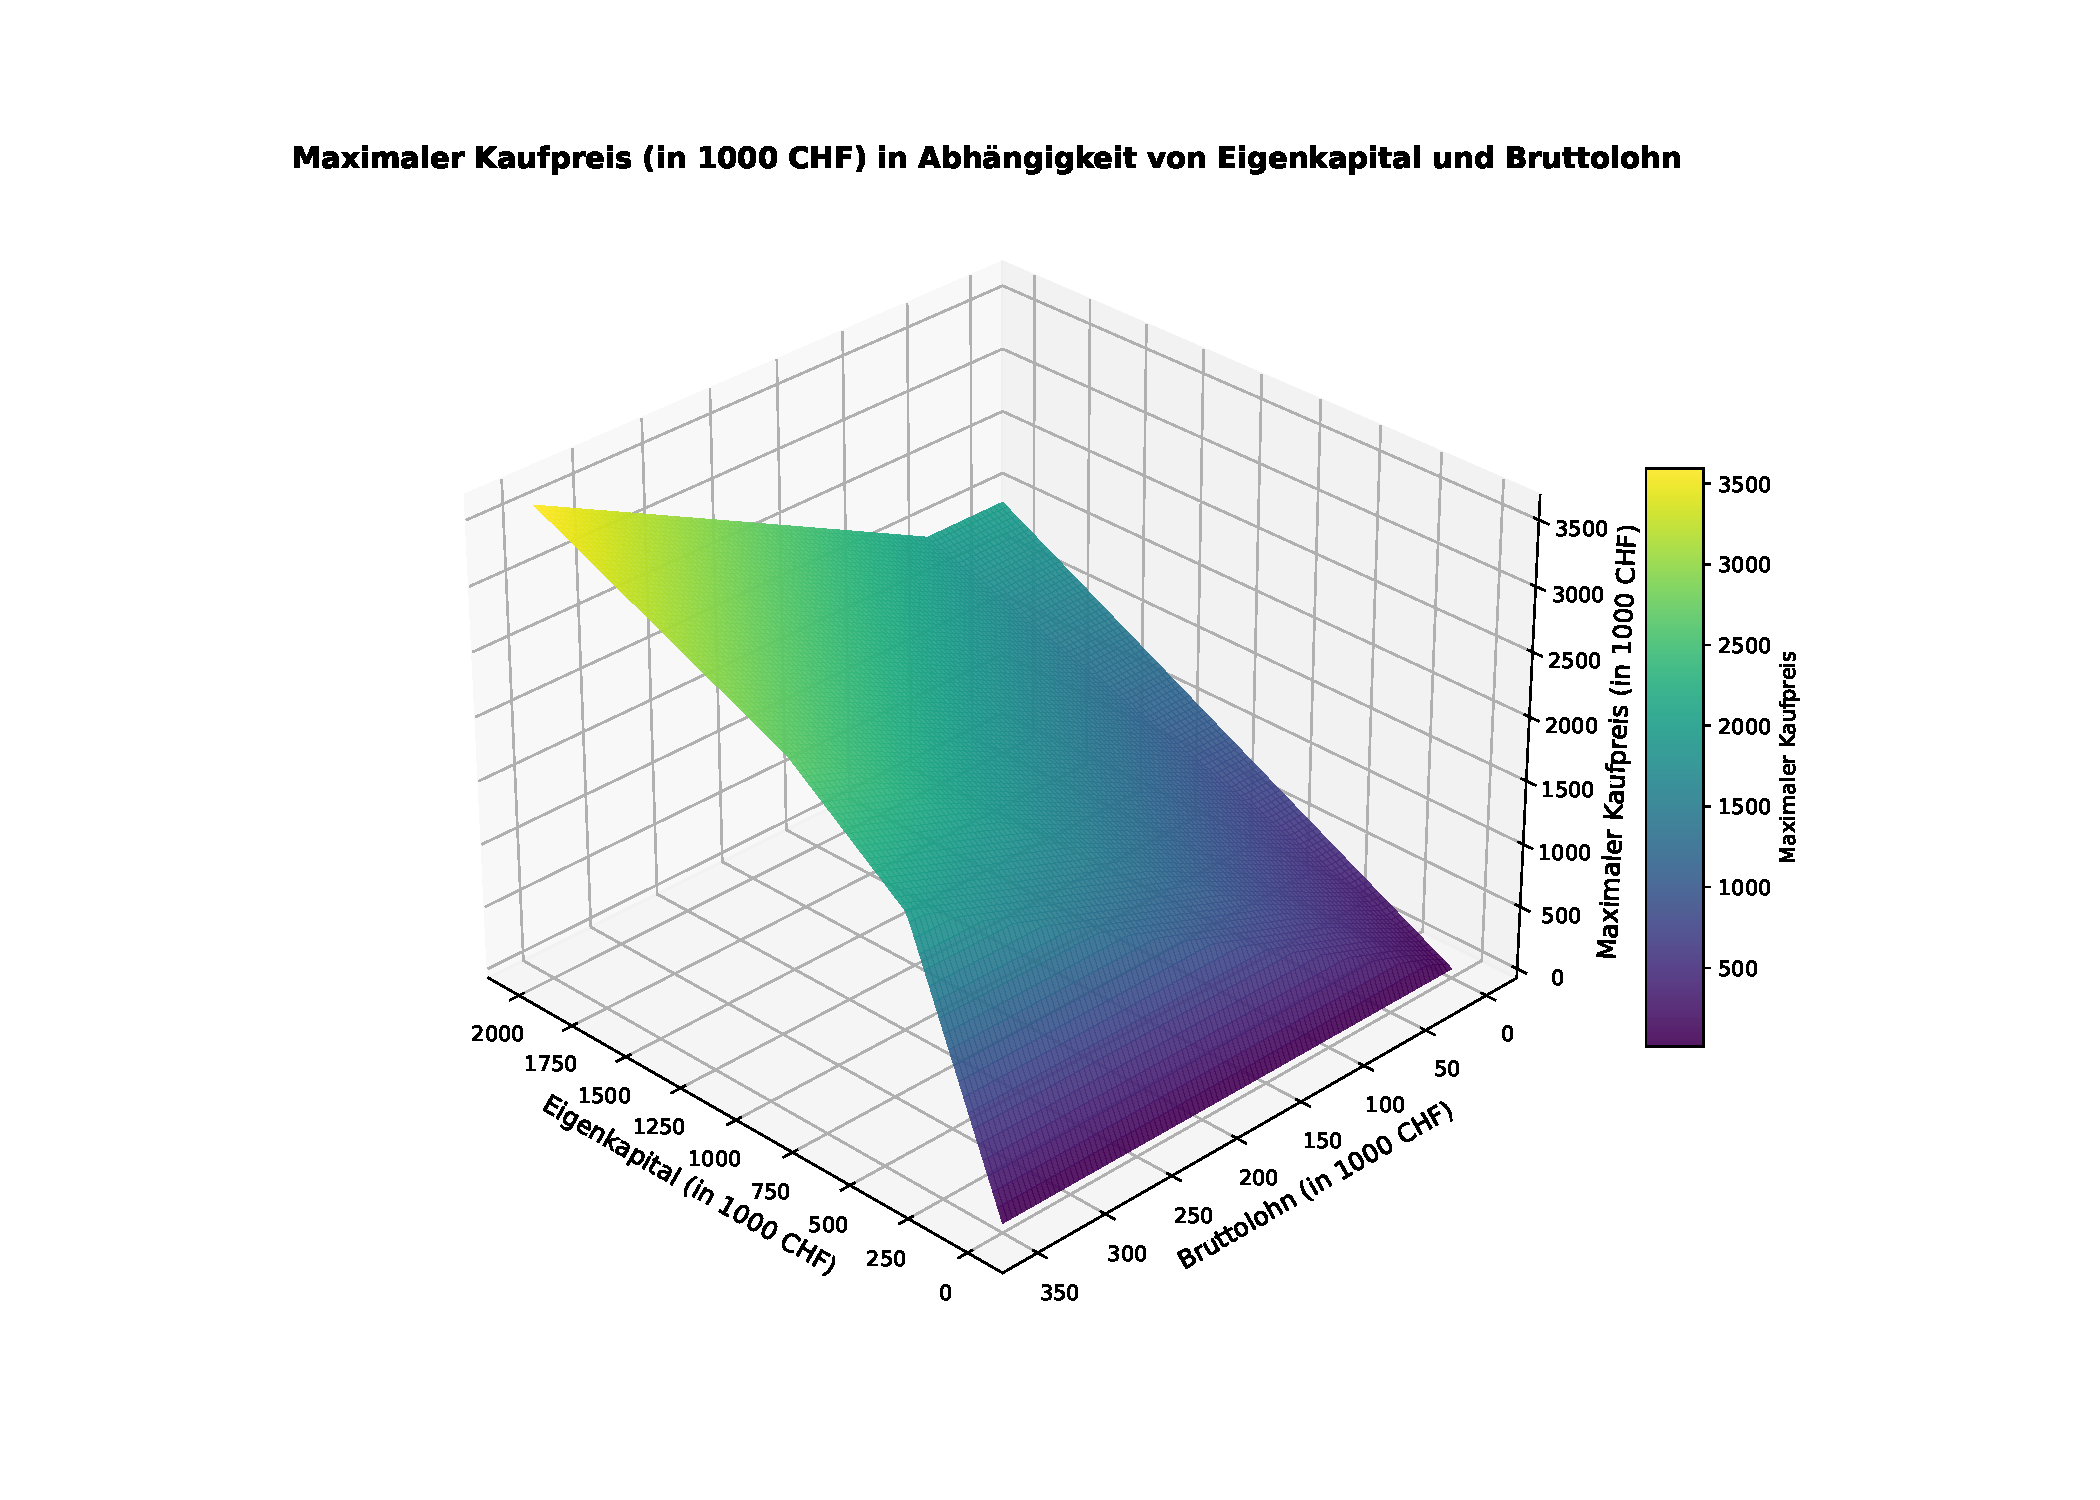
\includegraphics[width=0.9\textwidth]{Grundlagen_Info/00_Programmieren/Skript/Code/K04_Functions/max_kaufpreis_3d_plot.pdf}
% 		\caption{3D-Plot des maximalen Kaufpreises abhängig vom Jahresbruttolohn und dem Eigenkapital für $\alpha = 0.05, \beta = 0.01$.}
% 	\end{figure}

% 	\item Und schliesslich die Formel in Excel:

% 	\lstinline[basicstyle=\ttfamily\scriptsize]{MAX(MIN(MIN((A2/3 + A3 * A1) / (A3 + A4), (15 * A2 + 45 * A3 * A1 + 3 * A1) / (45 * A3 + 45 * A4 + 1)), 5 * A1), A1)}
% 	\end{enumerate}
% 	\end{myanswer}
% } %